\chapter{Theory}

\section{Gamma Radiation}
Unlike charged particles, which give off their energy through many interactions by either ionizing other atoms or elastic scattering, gamma rays tend to give off their energy in single bursts by the photoelectric effect (low energies), pair production (high energies) or \textit{Compton scattering} (intermediate energies).

In first order, this leads to a linear relationship between particle energy and distance travelled for charged particles. Thus, they can be shielded entirely.

On the other hand, gamma rays are either absorbed directly by the photoelectric effect or pair production or they change their direction by Compton scattering. Considering a detector pointing in the direction of incident flow, this implies that less gamma rays are detected if an absorber is present, however, gamma rays that do not interact with the absorber still retain their whole initial energy. Therefore, gamma radiation in matter loses intensity but not energy.

For the number of absorbed quanta $\d N$ per path length $\d x$ it holds
\begin{equation}\label{eq:dN}
	\d N = -\mu\cdot N(x)\d x,
\end{equation}
where $\mu$ denotes the \textit{absorption coefficient}.

Integrating \autoref{eq:dN} from 0 to the thickness $d$ of the absorber yields
\begin{equation}\label{eq:Nd}
	N(d) = N_0\cdot\e^{-\mu d},
\end{equation}
where $N_0\equiv N(x=0)$.

As expected, \autoref{eq:Nd} implies that gamma radiation may never be shielded of in its entirety.

\section{The Compton Effect}
\subsection{Differential Cross-Section}
\begin{figure}
	\centering
	\begin{subfigure}{0.49\textwidth}
		\centering
		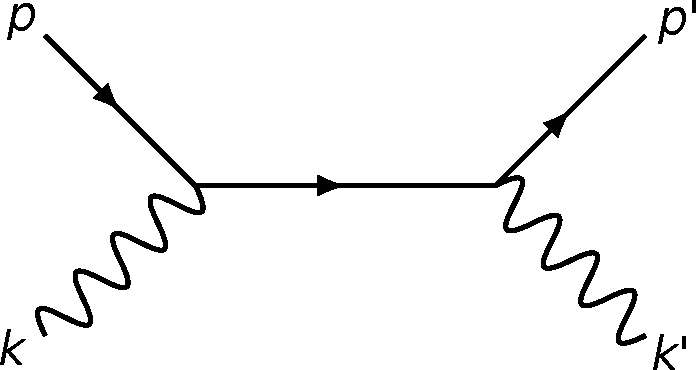
\includegraphics[width=\textwidth]{./img/s-channel.pdf}
		\caption{s-channel}
		\label{fig:schannel}
	\end{subfigure}
	\qquad\qquad
	\begin{subfigure}{0.2\textwidth}
		\centering
		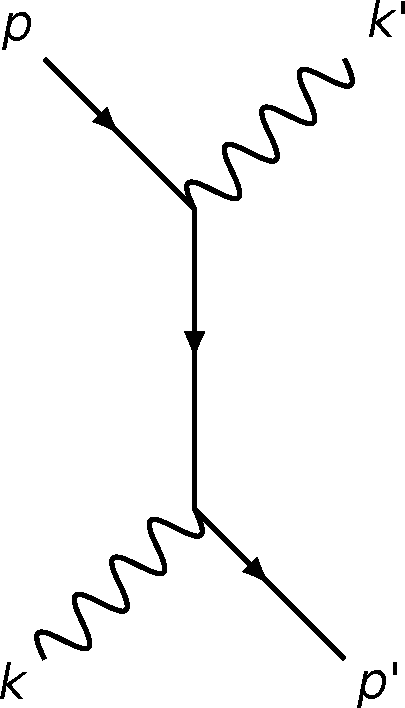
\includegraphics[width=\textwidth]{./img/t-channel.pdf}
		\caption{t-channel}
		\label{fig:tchannel}
	\end{subfigure}
	\par\bigskip
	\begin{subfigure}{0.45\textwidth}
		\centering
		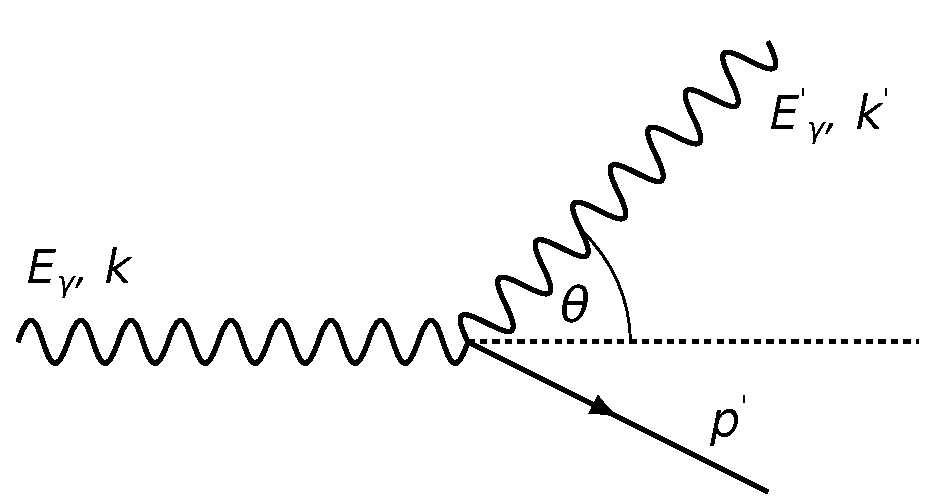
\includegraphics[width=\textwidth]{./img/kinematic.pdf}
		\caption{Kinematic sketch}
		\label{fig:kinematics}
	\end{subfigure}
	\caption{The two tree-level Feynman graphs contributing to the matrix element and a kinematic sketch for Compton scattering}
\end{figure}

The Compton effect is a scattering process of gamma quanta at a free, charged particle. At tree-level, two Feynman graphs (seen in Subfigures \ref{fig:schannel} and \ref{fig:tchannel}) contribute to the Feynman amplitude $\mathcal{M}$.
Denoting the respective 4-momenta of the incident photon and resting electron as
\begin{align*}
	k^\mu &= (k_0\ ,\ \mvec{k}) \\
	p^\mu &= (p_0\ ,\ \mvec{p}),
\end{align*}
and their 4-momenta after the process as primed, using the Feynman rules of QED, we get the two Feynman amplitudes

\begin{align*}
	\mathcal{M}_1 &= \bar{u}^{s'}\left(p'\right)\left(-\iu e\gamma^\nu\right)\epsilon^{*}_\nu\left(k'\right)\left(\frac{\slashed{p}+\slashed{k}+m}{(p+k)^2-m^2}\right)\left(-\iu e\gamma^\mu\right)\epsilon_\mu\left(k\right)u^s(p)\\
	\mathcal{M}_2 &= \bar{u}^{s'}\left(p'\right)\left(-\iu e\gamma^\nu\right)\epsilon_\nu\left(k\right)\left(\frac{\slashed{p}-\slashed{k}+m}{(p-k')^2-m^2}\right)\left(-\iu e\gamma^\mu\right)\epsilon^{*}_\mu\left(k'\right)u^s(p),
\end{align*}
where $u^s(p)$ denotes the incoming electron with spin $s$ and momentum $p^\mu$, $\epsilon^\mu$ is the incident photon's polarization vector and $\gamma^\mu$ are the Dirac matrices.

Since in the canonical formulation of QED the Feynman amplitudes represent terms in the Wick expansion of the perturbative scattering matrix, the total transition amplitude is equal to the sum of these matrix elements
\begin{equation*}
	|\mathcal{M}|^2 = |\mathcal{M}_1|^2 + |\mathcal{M}_2|^2 + 2\Re\left(\mathcal{M}_1\mathcal{M}_2^*\right).
\end{equation*}

For the sake of simplicity (and brevity!), we refer the reader to their QFT textbook of choice and just give the final result in the lab frame
\begin{equation}\label{eq:kleinnishina}
	\frac{\d\sigma}{\d\cos\theta} = \frac{\pi\upalpha^2}{m^2}\left(\frac{\omega'}{\omega}\right)^2\left[\frac{\omega'}{\omega} + \frac{\omega}{\omega'} - \sin^2\theta\right],
\end{equation}
where $m\omega' = \frac{1}{2}\left(m^2-u\right)$ and $m\omega = \frac{1}{2}\left(s-m^2\right)$ and $s=\left(p^\mu + k^\mu\right)^2, s=\left(p^\mu + k'^\mu\right)^2$ are the standard Mandelstam variables.
\autoref{eq:kleinnishina} is known as the \textit{Klein-Nishina formula}.

For electrons bound in an atom, the total cross-section is (in first order) proportional to its atomic number $Z$
\begin{equation*}
	\sigma = Z\cdot\sigma_\text{e}.
\end{equation*}
\subsection{Kinematics}
Consider initial
\begin{align*}
	p^\mu &= (m\ ,\ \mvec{0}) \text{and}\\
	k^\mu &= (E_\gamma\ ,\ \mvec{k})
\end{align*}
and scattered 4-momenta
\begin{align*}
	p'^\mu &= (m\ ,\ \mvec{p}) \text{and}\\
	k'^\mu &= (E'_\gamma\ ,\ \mvec{k'}).
\end{align*}
Using energy
\begin{equation*}
	m + E_\gamma = E'_\text{e} + E'_\gamma,
\end{equation*}
and momentum conservation
\begin{equation*}
	p^2 = E_\text{e}^{'2} - m^2 = \underbrace{E_\gamma^2 + E_\gamma^{'2} - 2E_\gamma E'_\gamma\cos\theta}_\text{law of cosines},
\end{equation*}
yields the energy of the scattered gamma ray
\begin{equation*}
	E'_\gamma = \frac{E_\gamma}{1 + \frac{E_\gamma}{m}\left(1 - \cos\theta\right)}
\end{equation*}
where $E'_\text{e}$ denotes the electron's total energy after the scatter process.
